\section{Imagination Augmented Agent (I2A)} 
\label{sec:i2a} 
 
The paper "Imagination-augmented agents for deep reinforcement learning" from Weber et al. \cite{I2A} combines the advantages of model free and model based reinforcement learning to get an agent which is robost against model imperfections but is able to use the advantages of model based agents.
The imagination-augmented agent learns therefore to combine information from a model-free and a model-based imagination-augmented path.\\

%To do this they train a model of the environment for internal simulations. 
%Imagine the future and learn to do better actions based on the imagined future.\\ 
 
Figure \ref{fig:i2a_architecture} shows the network architecture of the imagination-augmented agent, which will be explained in the following.

\begin{figure}[H] 
  \centering 
   
  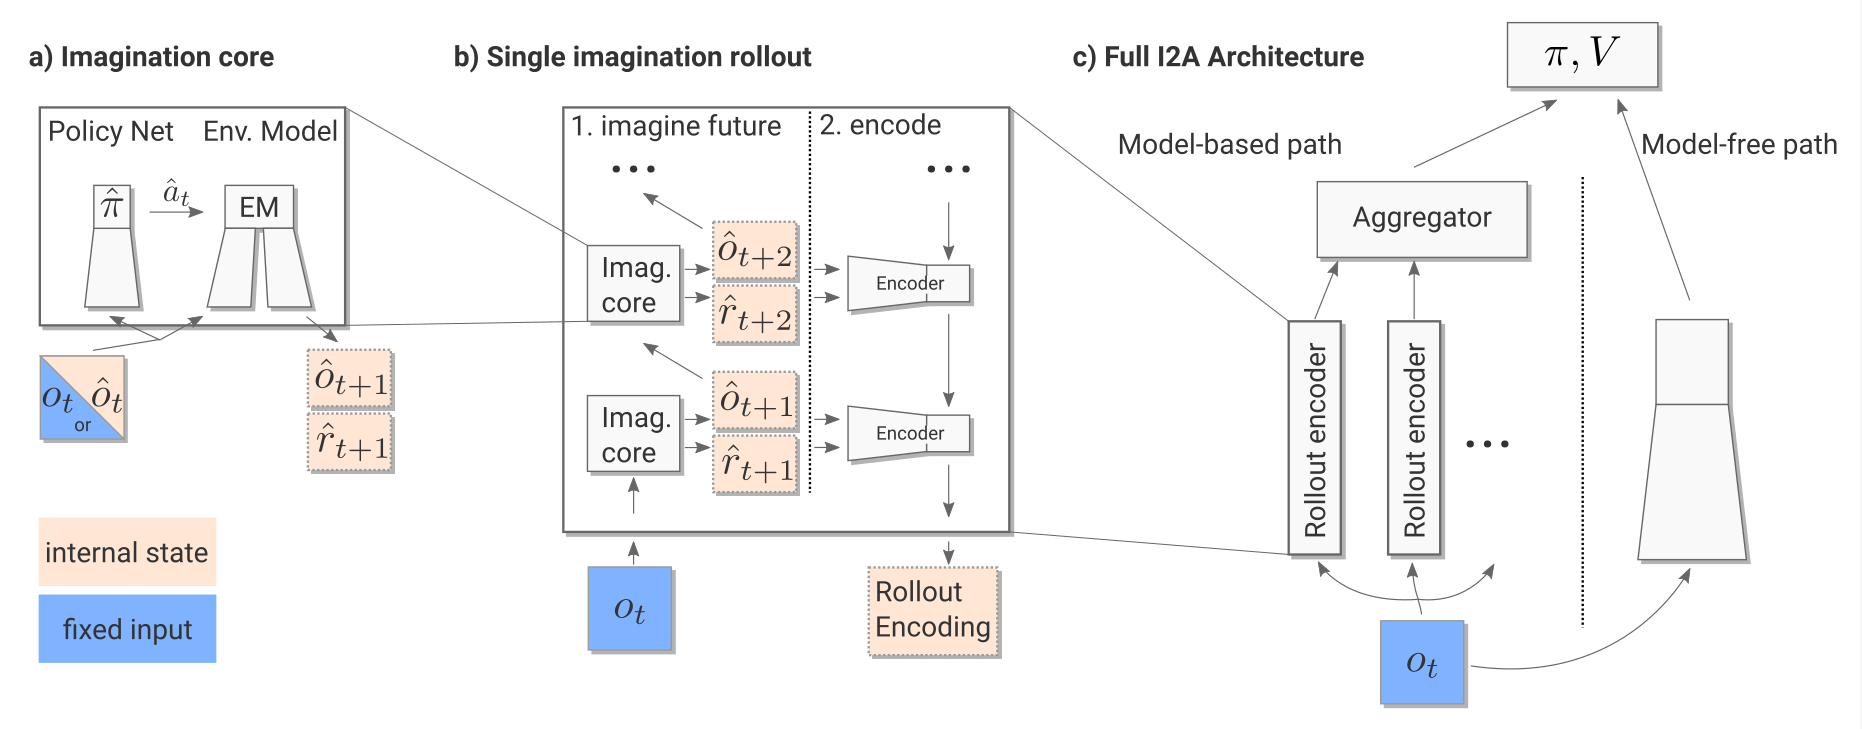
\includegraphics[width=\columnwidth]{./Images/i2a_architecture.png} 
  \caption{Network architecture for deep reinforcement learning which combines model free and model based reinforcement learning. a) imagination core (IC) predicts the next time step conditioned on an action sampled from the rollout policy $\hat{\pi}$. b) the from the imagination core imagines trajectories of features f encoded by the rollout encoder. c) the full i2a} 
  \label{fig:i2a_architecture} 
\end{figure} 
 
\subsection{Imagination core}

%The \textbf{imagination core} (Figure \ref{fig:i2a_architecture} a) imagine the next observation $\hat{o}_{t+1}$ and the next reward $\hat{r}_{t+1}$ given the observation $o_t$ or $\hat{o}_{t}$, where $o_t$ refers to the  input i2a get and $\hat{o}_{t}$ refers to an internal state of i2a which is an output of a previouse rollout with the imagination core. The pair of next observation $\hat{o}_{t+1}$ and the next reward $\hat{r}_{t+1}$ is called features $\hat{f} = (\hat{o}, \hat{r})$\\

The \textbf{imagination core} (Figure \ref{fig:i2a_architecture} a) imagine trajectories of features $\hat{f}_{t+1} = (\hat{o}_{t+1}, \hat{r}_{t+1})$, containing the next observation $\hat{o}_{t+1}$ and the next reward $\hat{r}_{t+1}$, given the observation $o_t$ or $\hat{o}_{t}$, where $o_t$ refers to the  input i2a get and $\hat{o}_{t}$ refers to an internal state of i2a which is an output of a previouse rollout with the imagination core.
To do so the imagination core uses a rollout policy, which predict an action given the current state, and an environment model see chapter \ref{sec:env_model}, which predict the next observation and the next reward.\\

%$o_t$: initial observation  $\hat{o}_t$: predicted observation  $\hat{r}_t$: predicted reward Given observation $o_t$ or $\hat{o}_t$ and action $\hat{a}_t$ predict (imagine) the next observation $\hat{o}_{t+1}$ and next reward $\hat{r}_{t+1}$  

%To do so the imagination core uses a rollout policy, which decides the next action $\hat{a}_t$, and an environment model, which predicts the next state and the reward signals from the environment, given an state and a current action.\\


The \textbf{rollout policy $\hat{\pi}$} is a model-free reinforcement learning agent which should, given the same observation, predict the same action as the i2a policy. To ensure this, the rollout policy need to be similar to the i2a policy $\pi$, which can be ensure by minimizing the distillation loss, the cross entropy between the rollout policy $\hat{\pi}$ and the i2a policy $\pi$:

%Distillation loss Make $\hat{\pi}$ (rollout policy) and $\pi$ (i2a policy) similar\\ 
 
\begin{equation} 
    l_{dist}(\pi, \hat{\pi})(o_t) = \lambda_{dist} \sum_a \pi(a | o_t) log \hat{\pi}(a|o_t) 
\end{equation} 

with scaling parameter $\lambda_{dist}$.
% $\lambda_{dist}$ is set to 10


 
\subsection{Rollout Encoder}
 

The rollout encoder processes the imagined rollout as a whole and learns to interpret it, by using any usful information or ignoring information when necessary, see Figure \ref{fig:i2a_architecture}b.\\

To do so each rollout encoder predicts a imagined trajectory $T = (\hat{f}_{t+1}, ... \hat{f}_{t+n})$, which is a sequence of features, by performing $n$ rollouts, given the input observation $o_t$ and a start action $a_t$.
%To do so each rollout encoder gets as input the input observation $o_t$ and a start action $a_t$ and performs $n$ rollouts by predicting a sequence of n features $\hat{f}_{t+i} = (\hat{o}_{t+i}, \hat{r}_{t+i})$ for $i = 0,...n$, this sequence of features $(\hat{f}_{t+1}, ... \hat{f}_{t+n})$ is called a imagined trajectory $T$.\\
The encoder constient of a CNN network following by a LSTM network which processes the information given by the imagined trajectory $T$. By using a LSTM network the encoder is able to learn long-term dependencies in the rollouts.

 
%The imagination core imagines trajectories of features $f = (\hat{o}, \hat{r})$\\ 
%The rollout encoder encode these trajectories     
%CNN Network followed by an LSTM Network 
%CNN Network:    Encode observation and reward $\hat{o}_{t+i}, \hat{r}_{t+i}$ 
%LSTM Network:    Learns long-term dependencies 
   
 
\subsection{I2A Architecture}


As described above the I2A architecture combines model free and model based reinforcement learning.
The model based path performs for each action $a$ the agent can take a imagination rollout with the rollout encoder.
The aggregator then concatinate all rollouts.
The model free path in contrast is just a neuronal network with CNN Layers followed by fully connected layers.
If only the model-free path would be used the architecture would be equal to a advantage-actor-critic architecture.\\
 

The outputs of the model-free path and the model-based path are then simple concatinated and passed to a output policy network which consists of one fully connected layer and two heads, the policy head $\pi$ and the value head $V$.
As I2A is just an architecture design it can be trained with advantage-actor-critic as described in section \ref{sec:a2c}.
The I2A architecture is trained as 

%For each action $a$ the agent can take do a imagination rollout  
% the future based on a model of the environment and use this information for decision making 
 
 
%I2A Architecture - Model Based Path  For each action $a$ the agent can take, do a imagination rollout     Aggregator:   Concatinate all action rollouts    

%I2A Architecture - Model Free Path CNN Layers followed by Fully Connected Layers 

 
%I2A Training 
%Input: Observation $o_t$ 
%Output:  Policy $\pi$ and value function $V$   Train with Advantage-Actor-Critic (A2C) 

\subsection{Environment Model (EM)}
\label{sec:env_model}

The environment model predict (imagine) the next observation $\hat{o}_{t+1}$ and next reward $\hat{r}_{t+1}$, given observation $o_t$ or $\hat{o}_t$ and action $\hat{a}_t$.
The environment model could be any kind of model that fullfills this condition, but in most cases no model of the enviroment is given.
To solve this problem the environment model is also a trainable neuronal network.
%, which is trained with enrolled pairs of (state, action) transitions made in the environment the i2a agent will act on.\\
A trained environment model can not be assumed to be perfect, it might sometimes make wrong prediction, but this does not matter as the imagination augmented agent is robust to imperfect environment models.

   
\begin{figure}[H] 
  \centering 
   
  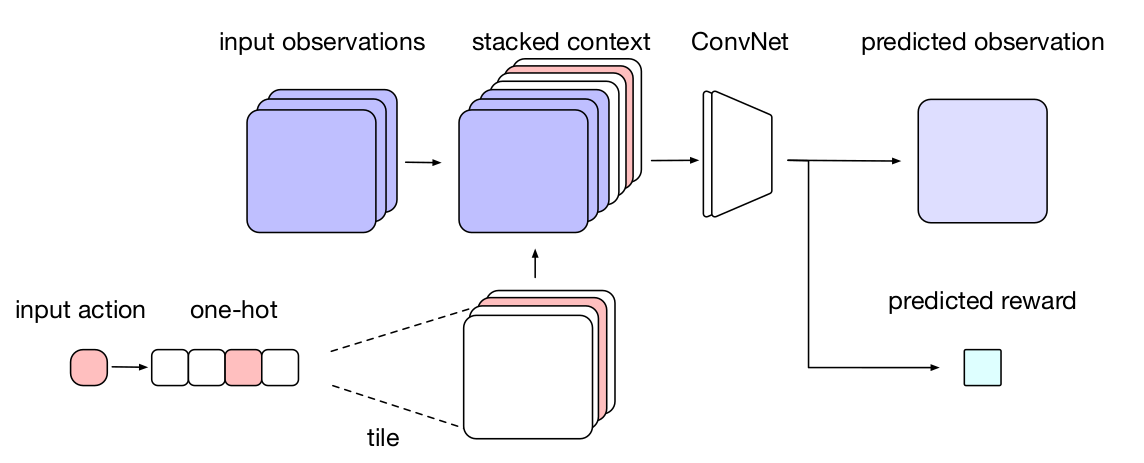
\includegraphics[width=300px]{./Images/environment_model_architecture.png}
  \caption{TODO} 
  \label{fig:environment_model_architecture} 
\end{figure} 

Figure \ref{fig:environment_model_architecture} shows the environment model architecture.
It gets as input the last observation $o_t$ as rgb image and a from the rollout policy $\hat{\pi}$ selected action $a$. The action is converted into a one hot vector and tiled to the size of the observation.
The tiled action is then concatinated with the input observations $o_t$.
The stacked context has now number of channels equal to three rgb channels plus the number of possible actions.
Given the stacked context as input a convolutional neural network with two heads predicts then the next observation $o_{t+1}$ and the expected reward $r_{t+1}$.\\

The neuronal network is trained with transitions of the form $(o_t, a_t) \rightarrow (o_{t+1}, r_{t+1})$ generated from a pretrained model-free advantage-actor-critic policy. This is nessesary because a random agent is not able to generate a representative set of states, as it sees few rewards in some of the domains.\\

 
The observation head of the environment model is trained by maximize the log likelihood of the probability $p(o_t | a_{t-1}, o_{t-1})$.
Where $p(o_t | a_{t-1}, o_{t-1})$ is a bernoulli distribution: 
\begin{equation} 
   p(o_t | a_{t-1}, o_{t-1}) = x^y (1-x)^{1-y} 
\end{equation}

A bernoulli distribution works well because \textbf{TODO}\\

%Basically we pretend that x and \hat x are both a collection of independent bernoulli probabilities (even if they are really just number in between 0 and 1).
   
Maximizing the log likelihood of the probability $p(o_t | a_{t-1}, o_{t-1})$ is the same as the binary cross entropy loss between the true image and the predicted image:

%The loss for training the observation of the environment model is therefor the same as the binary cross entropy between the true image and the predicted image:
   
\begin{equation} 
  \mathnormal{ 
  L_{env}(x, y) = \frac{1}{N} \sum y_n log x_n + (1-y_n) log(1- x_n) 
  %env_{loss} = Binary Cross Entropy(predicted\_image, true\_images) 
  } 
\end{equation}

To train the predicted reward a L2 loss is used.
 
 

\subsection{Copy Model}